\input{beamer.macros}
\usepackage[english]{babel}
\usepackage{tikz}
\usepackage{xmpmulti}
\newcommand{\fadeitem}[2]{\item[]\uncover<#1>{#2}}
\title{Validating Neighborhoods}
\author{Forest Gregg}
\begin{document}
\mode*

\mode<all>{
\fullscreenimage{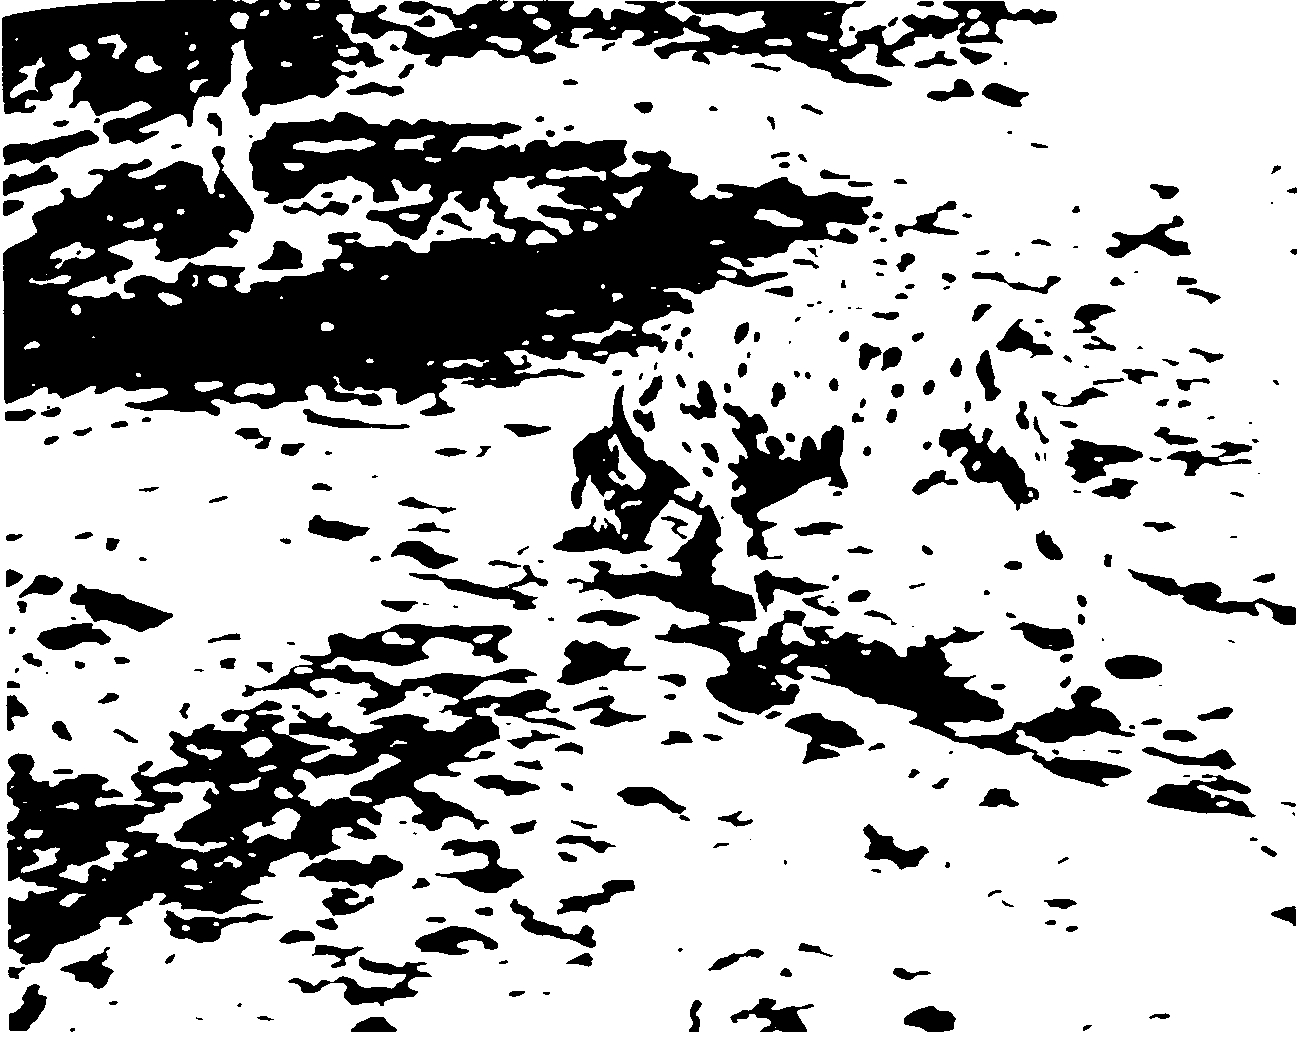
\includegraphics[width=\paperwidth]{./presentation_images/dog-park-big.jpg}}{Gestalt Dog}
}

\mode<all>{
\blackout{}
}  


\section{Introduction}
Today, I'd like to us to talk about a basic problem of social
research and some ideas about how we might respond. This is early
work, so I am going keep my presentation to short so we can talk.

So, here's the problem. In the social sciences, most of us study
aggregate things, like organizations, political parties, social
movements, or markets. In order to get on with that studying, we have
to decide what part of the world \emph{is} that thing that we are
studying.

\mode<all>{
\fullscreenimage{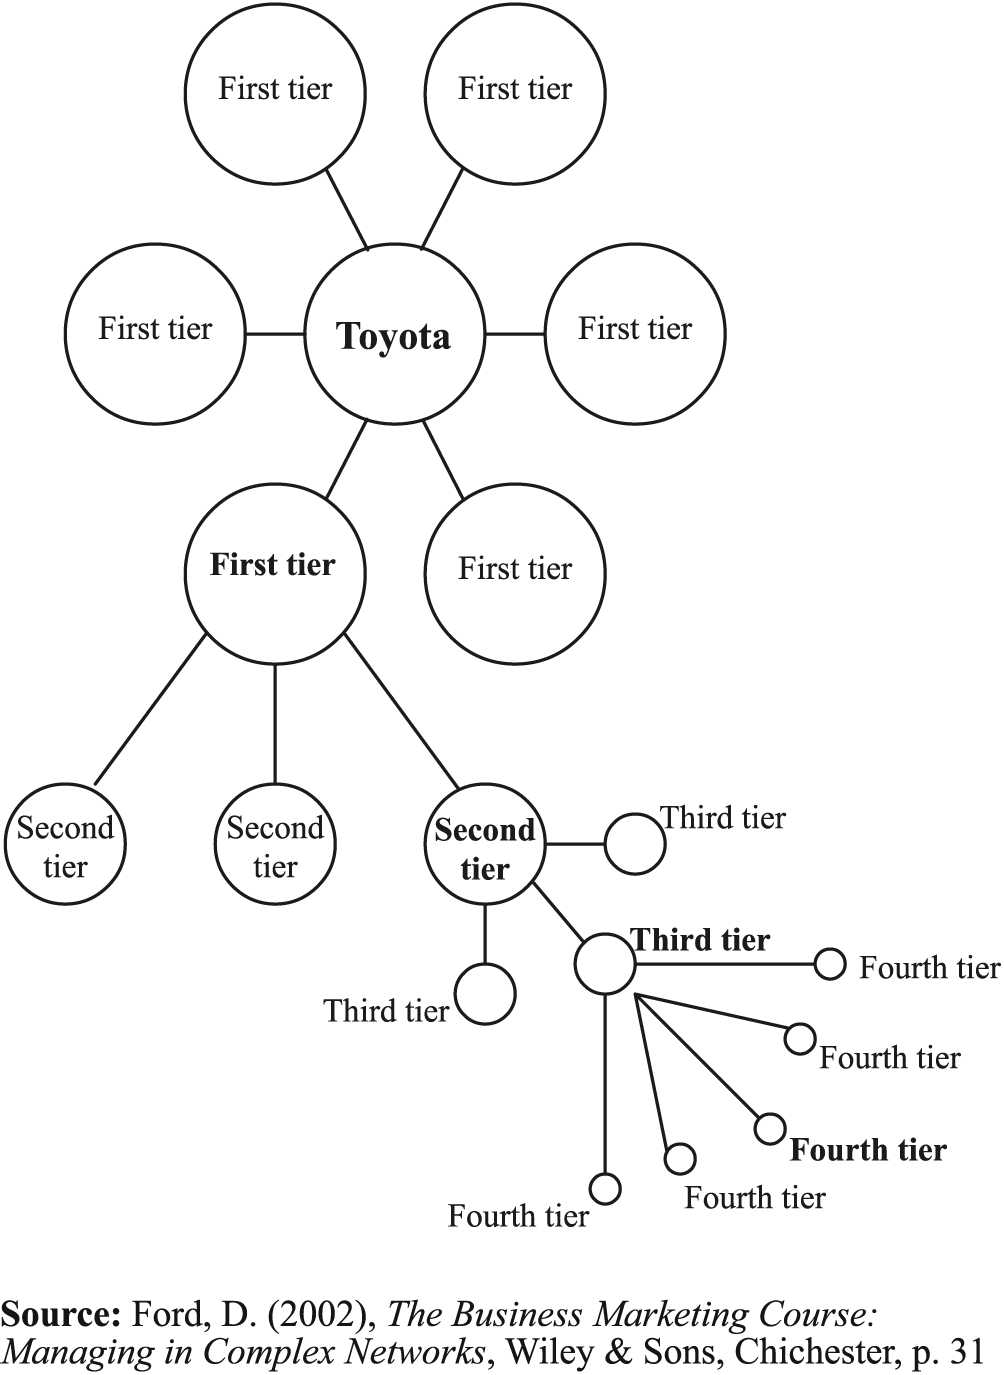
\includegraphics[height=\paperheight]{./presentation_images/toyotaSupply.png}}{Toyota}
}

If you want to study organizations, you have to decide what set of
entities and interactions are part of a particular organization and
which are not.

\mode<all>{
\fullscreenimage{
\includegraphics[width=\paperwidth]{./presentation_images/99-percent.jpg}}{Occupy Wall St.}
}


If you want to study social movements, you have to decide how who is
and is not part of the movement?

\mode<all>{
\fullscreenimage{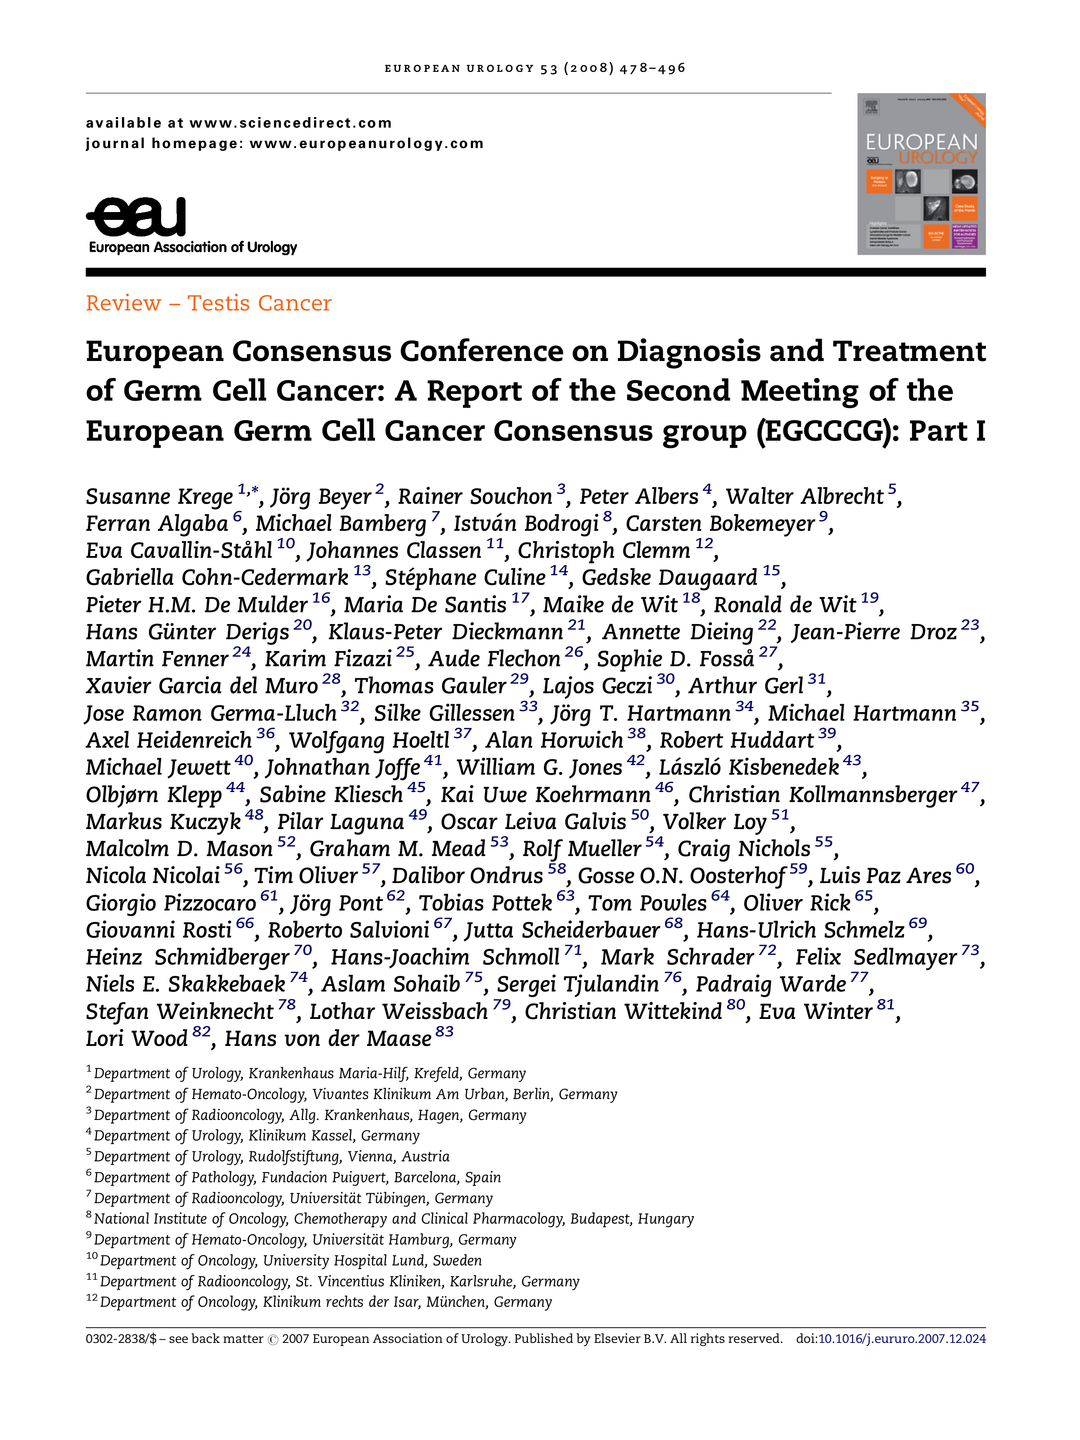
\includegraphics[height=\paperheight]{./presentation_images/many-author.png}}{Lots of Authors}
}

If you are studying scientific collaboration networks, you have to
decide what counts as a collaboration. Is it co-authorship?


\mode<all>{
\blackout{}
}  

For empirical research, we \emph{have} to divide up the world. But, if we
do that badly, then no degree of care of observation or sophistication
of technique can save us from drawing wrong conclusions about the
thing that we set out to study.

So, how do we make sure we don't do that? If we have to draw some
boundaries, then

\begin{frame}
\begin{center}
How do we know that we have gotten the boundaries right?
\end{center}
\end{frame}

That's what I want your help thinking about. For that conversation,
I'd like to review a concrete case. If we look at how some smart
people have tried to find good boundaries for a particular kind of
thing; that may be help us think.

Let's consider the neighborhood, and even more concretely, let's
consider \emph{how} social scientists have attempted to identify the
neighborhoods of Chicago over the past 100 years. 

If we do that, then even though there have been many different ideas
about what a neighborhood is, we can find some general agreement about
how we might know a neighborhood if we saw it. We've tended to think
that neighborhoods have these characteristics:

\section{Recognizing Neighborhoods}

\begin{frame}
Recognizing neighborhoods
\begin{itemize}
\item[] Neighborhoods are contiguous areas.
\pause
\item[] Inside neighborhoods, near things have more influence than distant things.\pause ..
\item[] ...for some set of social processes.  
  \mode<article>{
    \begin{itemize}
    \item[] If I keep my lawn neat, my neighbor may be more likely
      to keep her lawn neat, but the state of my lawn has much less
      influence on the number of beer cans on a lawn two streets over.
      
      The idea here is that neighborhoods hang together because the
      elements are all connected to their neighboring elements, and
      those elements are connected to their neighboring elements, etc.
      
      Alternatively, you could think that neighborhoods might hang
      together because the elements of a neighborhood are
      within some container, but the individual elements do not have any
      real relation to one another, like gas in a balloon. 
      
      Although some sociologists have focused more on containment,
      particularly in the case of legally enforced racial segregation,
      we have tended to think that within a neighborhood things go
      together because they are connected to each other.
    \end{itemize}
}
\pause
\item[] Across the boundaries of a neighborhood,
\begin{itemize}
\item[] Near things have much less influence on each other
\item[] Or, the sign of that influence changes. 
  \mode<article>{
    \begin{itemize}
    \item[] Let me explain that a little. Say that we are in
      postwar Chicago at the border between a black and white
      Southside neighborhoods. If a black family moved into the white
      neighborhood, but right at the edge, this tended to make white
      neighbors move \emph{away} from the black family, and to make
      the black neighbors move \emph{towards} it. In both cases, the
      neighbors were very much influenced, but that influence acted in
      different directions. 
    \end{itemize}
}
\end{itemize}
\end{itemize}
\end{frame}

\noindent This last property is the critical one. 

Just imagine we lived in a world where it was not true, and near
things are always more related than distant things, and that relation
always works in the same direction. If that is the world we lived in,
there could be enormous differences in the social geography of a
city. There could be areas that were all black and areas there were
all white. However, we should expect to see a region of mixing between
those areas. We should not expect to see sharp discontinuities.

In that world, trying to find a valid neighborhood would be like
trying to find the elevation when the foothills 'really' turn into
mountains. We should just say that a person's neighborhood is the area
within some radius around, say, their house.

\mode<all>{
\fullscreenimage{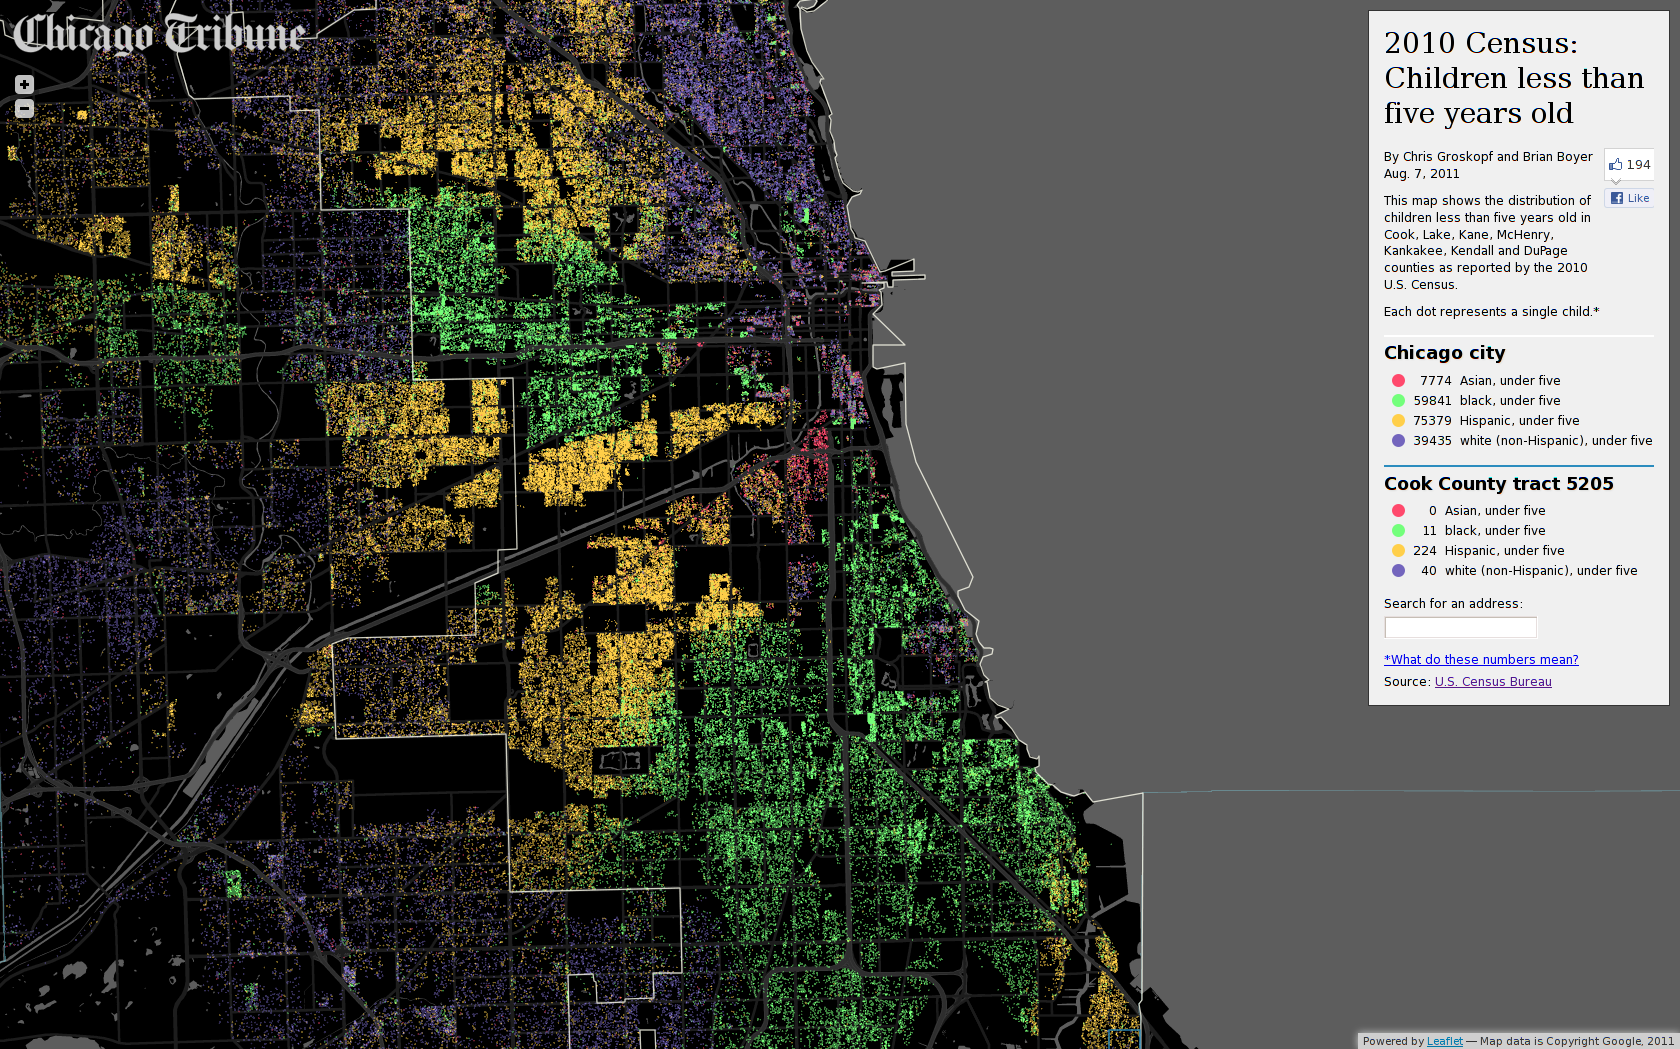
\includegraphics[width=\paperwidth]{./presentation_images/chicago_race.png}}{Chicago Race Map}
}

I don't think that's the world we live in, at least that's not the
city we live in. 


\mode<all>{
\blackout{}
}  

\section{Connectivity}

If this discontinuity is so important to the idea of a neighborhood,
we might try to start by identify these edges directly. Historically,
that is how we started.

\mode<all>{
\fullscreenimage{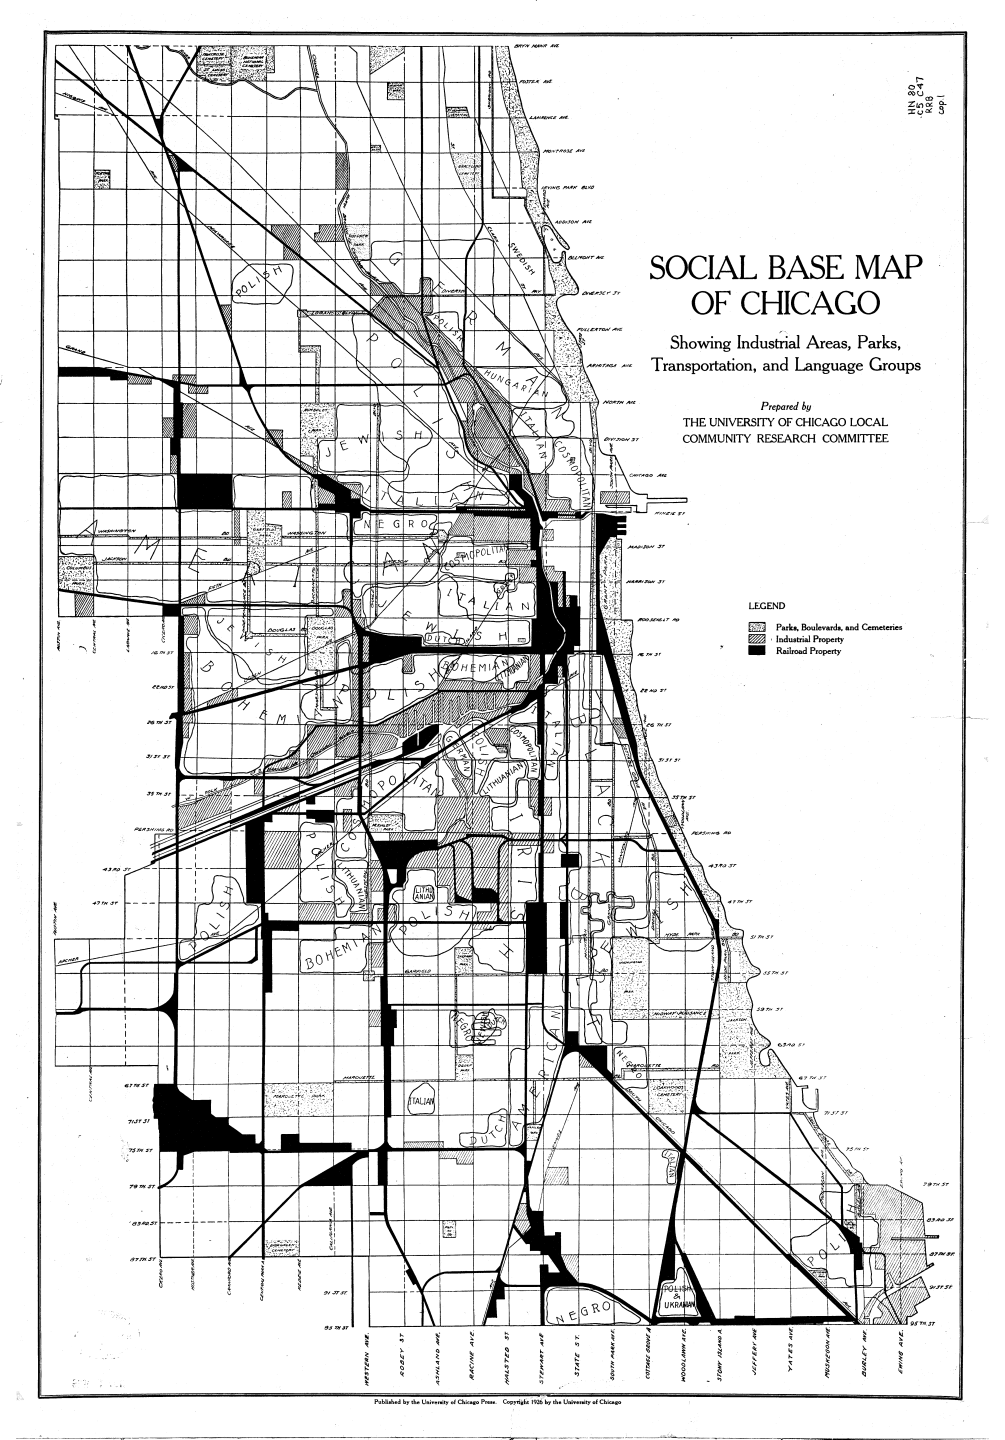
\includegraphics[height=\paperheight]{./presentation_images/comarea-0.png}}{Base Map}
}

In the 1920s, Ernest Burgess of our Department of Sociology had a map
made of Chicago showing rivers and canals, major street's, rail lines,
parks, and industrial areas. This map was used for a preliminary stage
of a grand research project that aimed to understand the principles
behind the physical growth of Chicago and the distribution of people
and land use through the city.

Vivian Palmer, Burgess's close collaborator on this work, summarizes
the vision:

\mode<all>{
\fullscreenimage{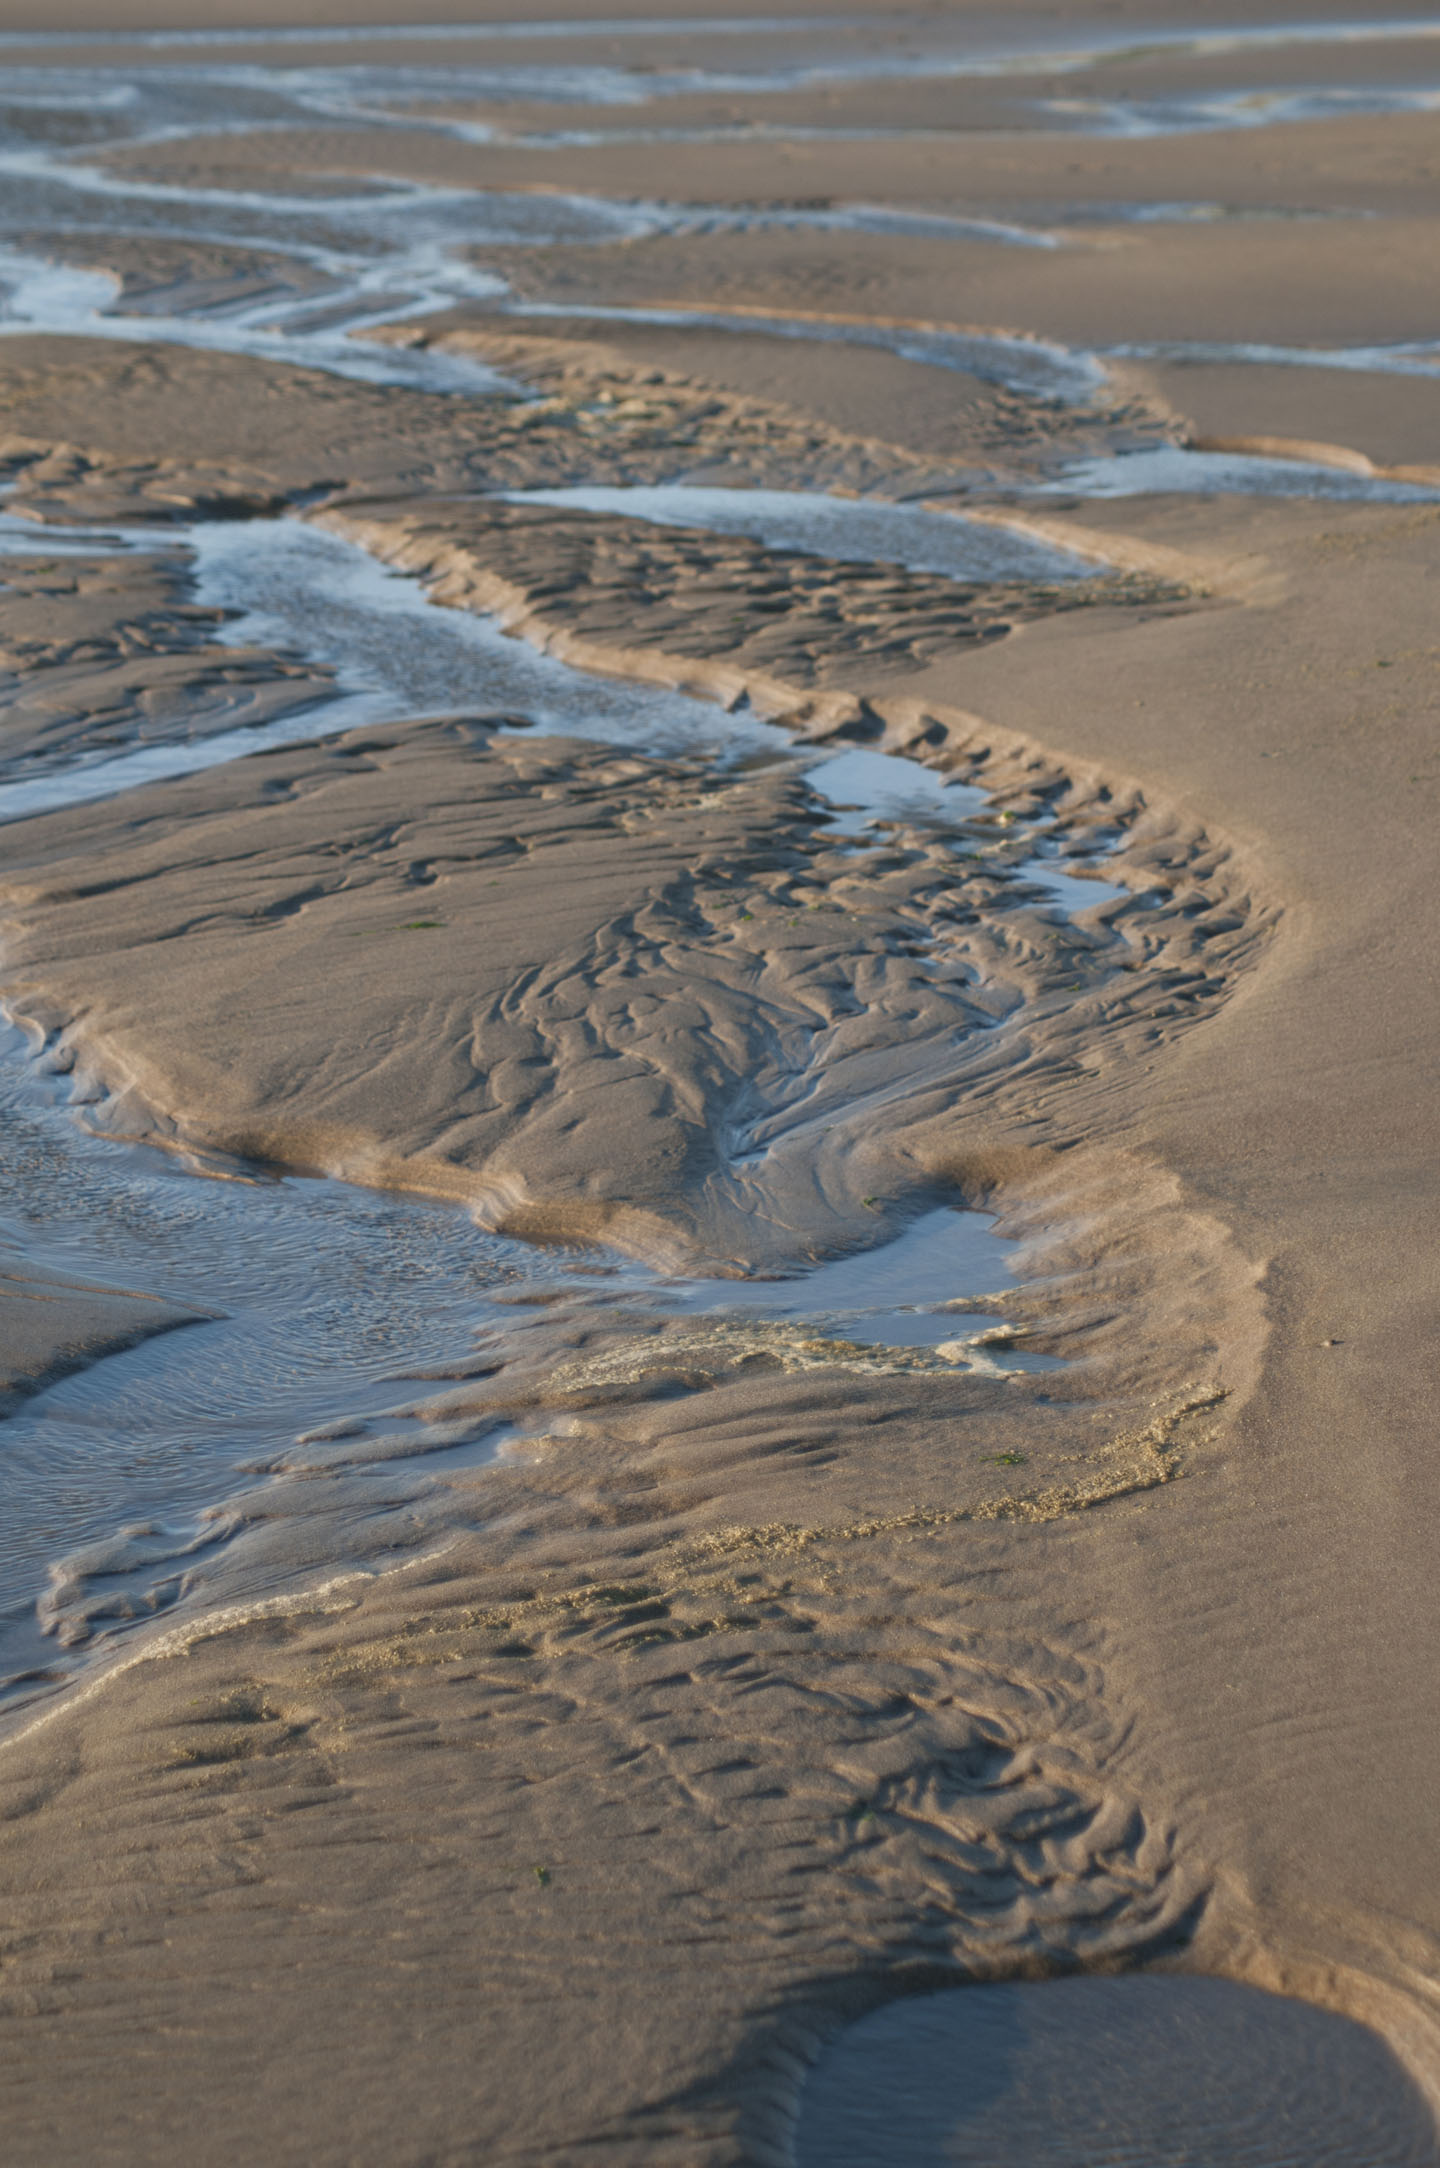
\includegraphics[height=\paperheight]{./presentation_images/smallOregonpuddle.jpg}}{Tidal Pools}
}


\begin{quote}
  It was assumed that the topographic and physical barriers erected by
  man gave the city a relief map with many small basins; [and] that
  competition for location regulated by land value sorted and
  distributed the population of the city into territorial groupings
  within these basins.
\end{quote}

\mode<all>{
\crossfade{png}{./presentation_images/comarea}{Base Map to Community Areas, 10 frames}

To identify these basins, Burgess looked for the barriers between
them. He reasoned that these physical features, which interrupted the
street grids, should constrict the flow of people between adjacent
areas. That is to say, reduce the relation between nearby things.

So, Burgess more or less squinted at this map, and split Chicago up
into 75 parts. He called these segments both ecological
areas and, unfortunately, ``Community areas,'' which would lead to
lots of confusion when people expected these areas to have something
to do with collective identity or neighborly interaction

One way of looking at what Burgess did is that he said neighborhoods
should follow the real street grid of a city.

\mode<presentation> {
  \begin{frame}<1>[label=valid_neighborhoods]
    Qualities of Valid Neighborhoods
    \begin{itemize}
    \item[]<1-> Neighborhoods should respect the street grid.
    \item[]<2-> Measures of neighborhood-scale social processes should
      be relatively homogeneous within neighborhoods.
    \item[]<3-> Neighborhoods should move as a unit.
    \item[]<4-> Residents should recognize neighborhoods.
    \item[]<5-> Neighborhoods should elemental or composed of elements
    \item[]<6-> Neighborhoods should be permitted to not exist
    \end{itemize}
  \end{frame}
}
\begin{figure}[h!]
\centering
\includeslide[height=5cm]{valid_neighborhoods<1>}
\end{figure}

I think that we might want to nominate that as a principle. Of course,
we cannot raise it to an absolute rule, as most of us would think that
the area east of the Metra tracks are still part of Hyde Park,
although that has sometimes not been perfect settled.

\section{Coelescence}

However, Burgess's division are very coarse. We know, as did
Burgess, that there are many distinct areas within these large
divisions of the city. Once we had social statistics at the
resolution of the census tract, we could attempt to
directly partition the city into relatively homogenous areas. In the
1930s, this is what Burgess, Charles Newcomb, and Philip Hauser did.

\mode<all>{
\fullscreenimage{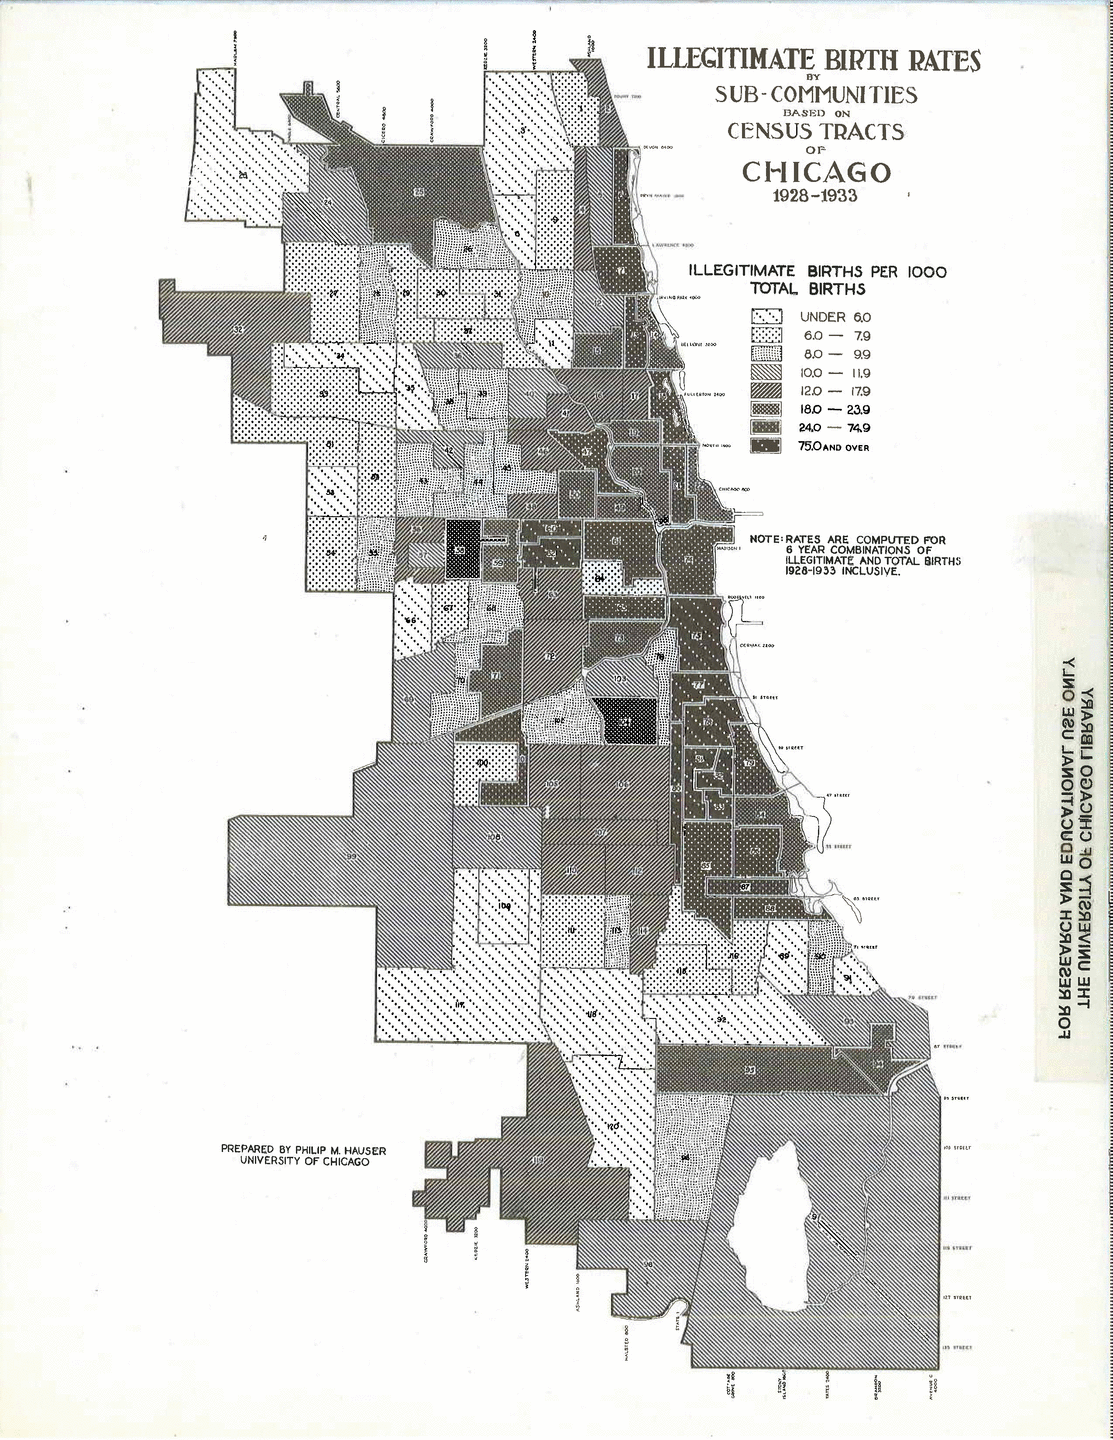
\includegraphics[height=\paperheight]{./presentation_images/hauser.png}}{Subcommunity areas}
}

Hauser describes his approach like this: 

\begin{quote}
The more important criteria employed in defining the areas were: the
equivalent median rental of the census tract, the nativity and race of
the population, the presence of physical barriers, the nature of the
transportation facilities, community and neighborhood tradition and
organization, and various indexes of social organization, particularly
the divorce rate and the delinquency rate. The investigators'
acquaintance with the city was also a factor
\end{quote}

Our own Professor Raudenbush took a very similar approach 60 years
later when he defined the ``Neighborhood Clusters'' for the Project on
Human Development in Chicago Neighborhoods.

So, we might want this to be our second principle: 

\againframe<2>{valid_neighborhoods}
\begin{figure}[h!]
\centering
\includeslide[height=5cm]{valid_neighborhoods<2>}
\end{figure}

\mode<all>{
\blackout{}
}    

\section{Moving Together}

The main problem with this approach is that it defines neighborhood
based upon measurements social processes, but only uses measurements
made at one point in time.

Defining a neighborhood well depends upon the idea that within a
neighborhood near things have more causal influence than distant
things. To get a feel for that causality, we are always better to see
how thing relate over time.

Burgess defined his ecological areas as a preliminary stage for an
enormous research project. He believed that if these areas were valid
divisions, then they should have somewhat independent developmental
histories, and he secured funding to study these `natural histories'
in a project called the ``Social History of Local Communities in
Chicago'' This project was directed by a graduate student named
Vivian Palmer. Starting in 1924, and for the next eight years, Palmer
organized the research of hundreds of undergraduate sociology students
and collected enormous volume of materials from civic organizations,
business associations, and governmental organs.

This is what she found:

\begin{quote}
  As our natural histories accumulated we began to realize that the
  ecological areas which had been defined mainly by topographic and
  economic criteria did not give us the elementary territorial
  groupings of the city. With our extensive research into these
  ecological areas we were finding that the majority of them contained
  a number of smaller territorial groupings which were often bound
  together at the present time by a common shopping and commercial
  center [and] which sometimes shared other institutions. Yet these
  units had other distinctive characteristics and group relationships,
  often subtle yet recognized by their residents, which set them apart
  from each other. So we sought to formulate some new conception which
  would enable us to explain the existence of these smaller groupings
  and delimit them objectively...

  A more careful examination of... the development of the natural
  territories led us to the conception of the primary settlement areas
  as the unit of our research.

  As Chicago expanded outward from its embryo village of a few square
  miles it grew decade by decade, and is still growing, by the
  addition of small relatively isolated settlements. With an abundance
  of open land always on its borders and under our present system of
  property ownership, small sections usually known as subdivisions
  were being placed on market for industrial, business, and home
  sites. As the city grew, also, its populations was becoming
  increasingly heterogeneous and groups relatively homogeneous in
  nationality, economic status, and occupational strata were becoming
  segregated in each of these new primary settlements. Most of these
  areas developed a local life and character.
\end{quote}

\begin{frame}
\begin{quote}
  Taken together they constituted a natural social organization of the
  city which was primary and over which many of the later forces of
  city growth had to work themselves over.
\end{quote}
\end{frame}


\mode<all>{
\crossfade{png}{./presentation_images/devel}{Development of Northside, 8 frames}
}

These settlements continue to pattern urban processes because, first,
sometimes, the residents are able organize together and resist the
processes of urban growth, but second, and more typically the
settlement's ``previous homogeneity insured its change practically as
a unit.''

These settlements would rarely coalesce, but could be split by
building a new barrier, like a railroad, belt of industry, public
park, or wide boulevard. However, even after a fire razed an area, she
claimed that primary settlement areas would re-emerge, and even when

\begin{frame}
\begin{quote}
[when] rooming houses appeared over several adjacent primary settlement
areas, like a chameleon, it took on the characteristics of the various
primary settlements beneath it, still showing perceptible difference
between the areas.
\end{quote}
\end{frame}

The key idea here is that the neighborhood is the thing that stays
together, that either does not change or changes as a unit.

\againframe<3>{valid_neighborhoods}
\begin{figure}[h!]
\centering
\includeslide[height=5cm]{valid_neighborhoods<3>}
\end{figure}

For Chicago and a number of other great American cities, we now have a
time series of tract level data going back eighty years. I have been
thinking about how we could use these data to find the parts of the
city that move together through socio-demographic state space, but I
have not figured out a good approach. I would love to hear any
thoughts about this in the conversation.

\section{Asking People}

Finally, I want to pick up on something that Palmer said. That her
`elemental territorial groupings' were recognized by residents. This
is I think the last principle, I would like to suggest today.

\againframe<4>{valid_neighborhoods}
\begin{figure}[h!]
\centering
\includeslide[height=5cm]{valid_neighborhoods<4>}
\end{figure}

There are two reasons why we should want residents to be able to
recognize neighborhoods. The first is that, if neighborhoods are
relatively distinct social areas of a city, then we should expect that
people who know those areas will tend to see them as distinct. The
second is that if residents see an areas as distinct area, that itself
is a socially meaningful way that the area differs from surrounding
areas, and one that may be very consequential to way an area develops
if people come to value the area and act upon those evaluations.

In the 1960s, Albert Hunter attempted to define neighborhoods based
upon asking Chicagoans two questions: ``What is the name of this part
of Chicago.'' and ``What are the boundaries of this area.''

\mode<all>{
\fullscreenimage{\includegraphics[height=\paperheight]{./presentation_images/hunter_areas.pdf}}{Symbolic Communities}
}

This approach has two problems. 

First, we know that people who are wealthier and have more education
are more likely to say that the area where they live has a name, and
also, separately, that people who live in areas where people are more
wealthy and have more education also more likely to say that the area
has a name.

If you define neighborhoods based upon how people label them, it
appears that richer people tend to live in smaller, defined areas, and
that poorer people live in larger, less defined areas. That may
actually be true, but we don't really understand why this pattern of
responses exist. It could be that poor people are just as likely to
live in distinct areas, but for some reason they are less likely to
have a name for that are.

Second, when you ask people to tell you the boundaries of their
neighborhood or to draw you a map of their neighborhood, they usually
can't. If you find two people who can draw you maps, the maps will
almost never completely agree. 

Typically when faced with such variation, we respond by averaging the
responses together to estimate the central tendency. However,
practically this would mean that we need a very large sample in order
to get a stable estimate given that the size of some named
neighborhoods are quite small. As far as I know, such a large sample
has never been drawn.

Now, while people usually can't tell you the boundaries of their
neighborhood, they can usually tell you where they are: eighty five
percent could in Hunter's sample. If we asked enough people where they
were, we could use the distribution of responses to find where people
were more likely to say they were in one neighborhood versus another.

Or at least that's what I have become convinced of. For the past year,
I have been collecting data that I hope is a reasonable proxy for
asking people ``What is the name of this part of Chicago.''

\mode<all>{
\fullscreenimage{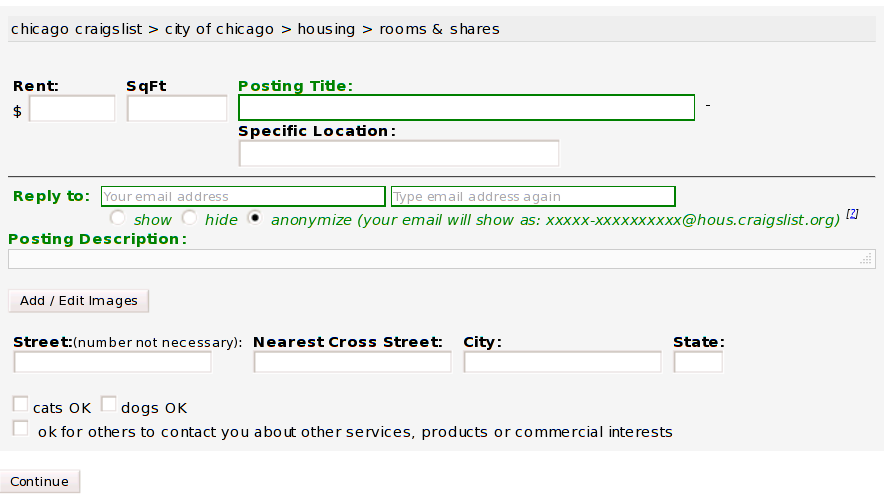
\includegraphics[height=60mm]{./presentation_images/craigslist.png}}{Craigslist entry form}
}

Every night, I download Craigslist apartment, rental, sublet and
roommate listings. When a persons posts a listing, they have the
option of putting in an address or intersection. This allows me to
associate latitude and longitude with a posting. They also have the
option of entering, in free text, the ``Specific location'' of the
posting.

People interpret ``Specific location'' in different ways, but most
people put in the name of a neighborhood.  With these data, I can
estimate how likely that a listing will say that a location is in the
neighborhood. I'm going to show you a map of the North Side where I
have the most data.

\mode<all>{
\fullscreenimage{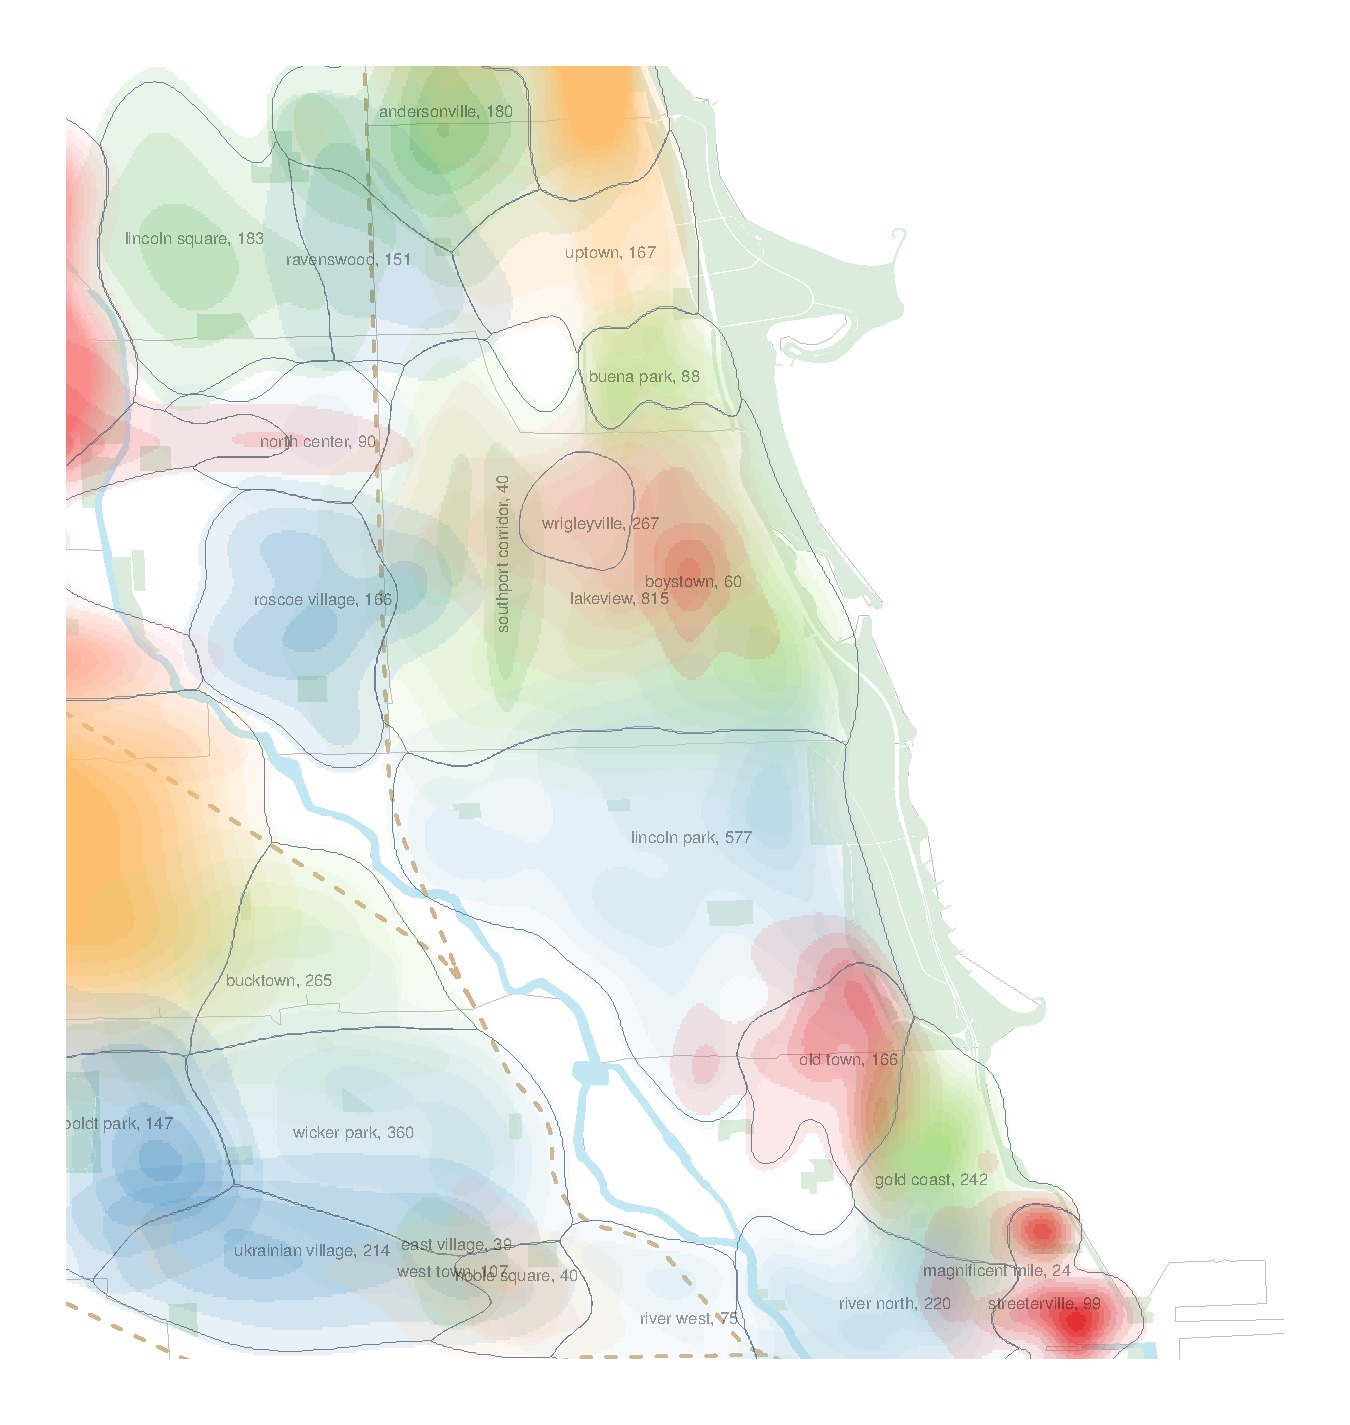
\includegraphics[height=\paperheight]{./presentation_images/ksplot.pdf}}{Kernel Density Plot}
}

The different colors represent correspond to different
neighborhoods. I estimated the probability using a kernel density
estimate, and the darker hues of a color correspond to a higher
probability that a poster will claim that location is in that
neighborhood. The swirly lines are where it becomes more likely that
someone will say that they are in one neighborhood versus another.

This is the river. These are rail-lines. These are parks. These gray
lines are the edges of Burgess's ecological areas. I think it's pretty
remarkable that, with the exception of Ravenswood and Old Town, and
maybe Andersonville, none of the neighborhoods cross any of the
borders he drew 90 years ago.

\mode<all>{
\mode<presentation>{	
  \begin{frame}[plain]
    \begin{tikzpicture}[remember picture,overlay]
      \node[at=(current page.center)] {
        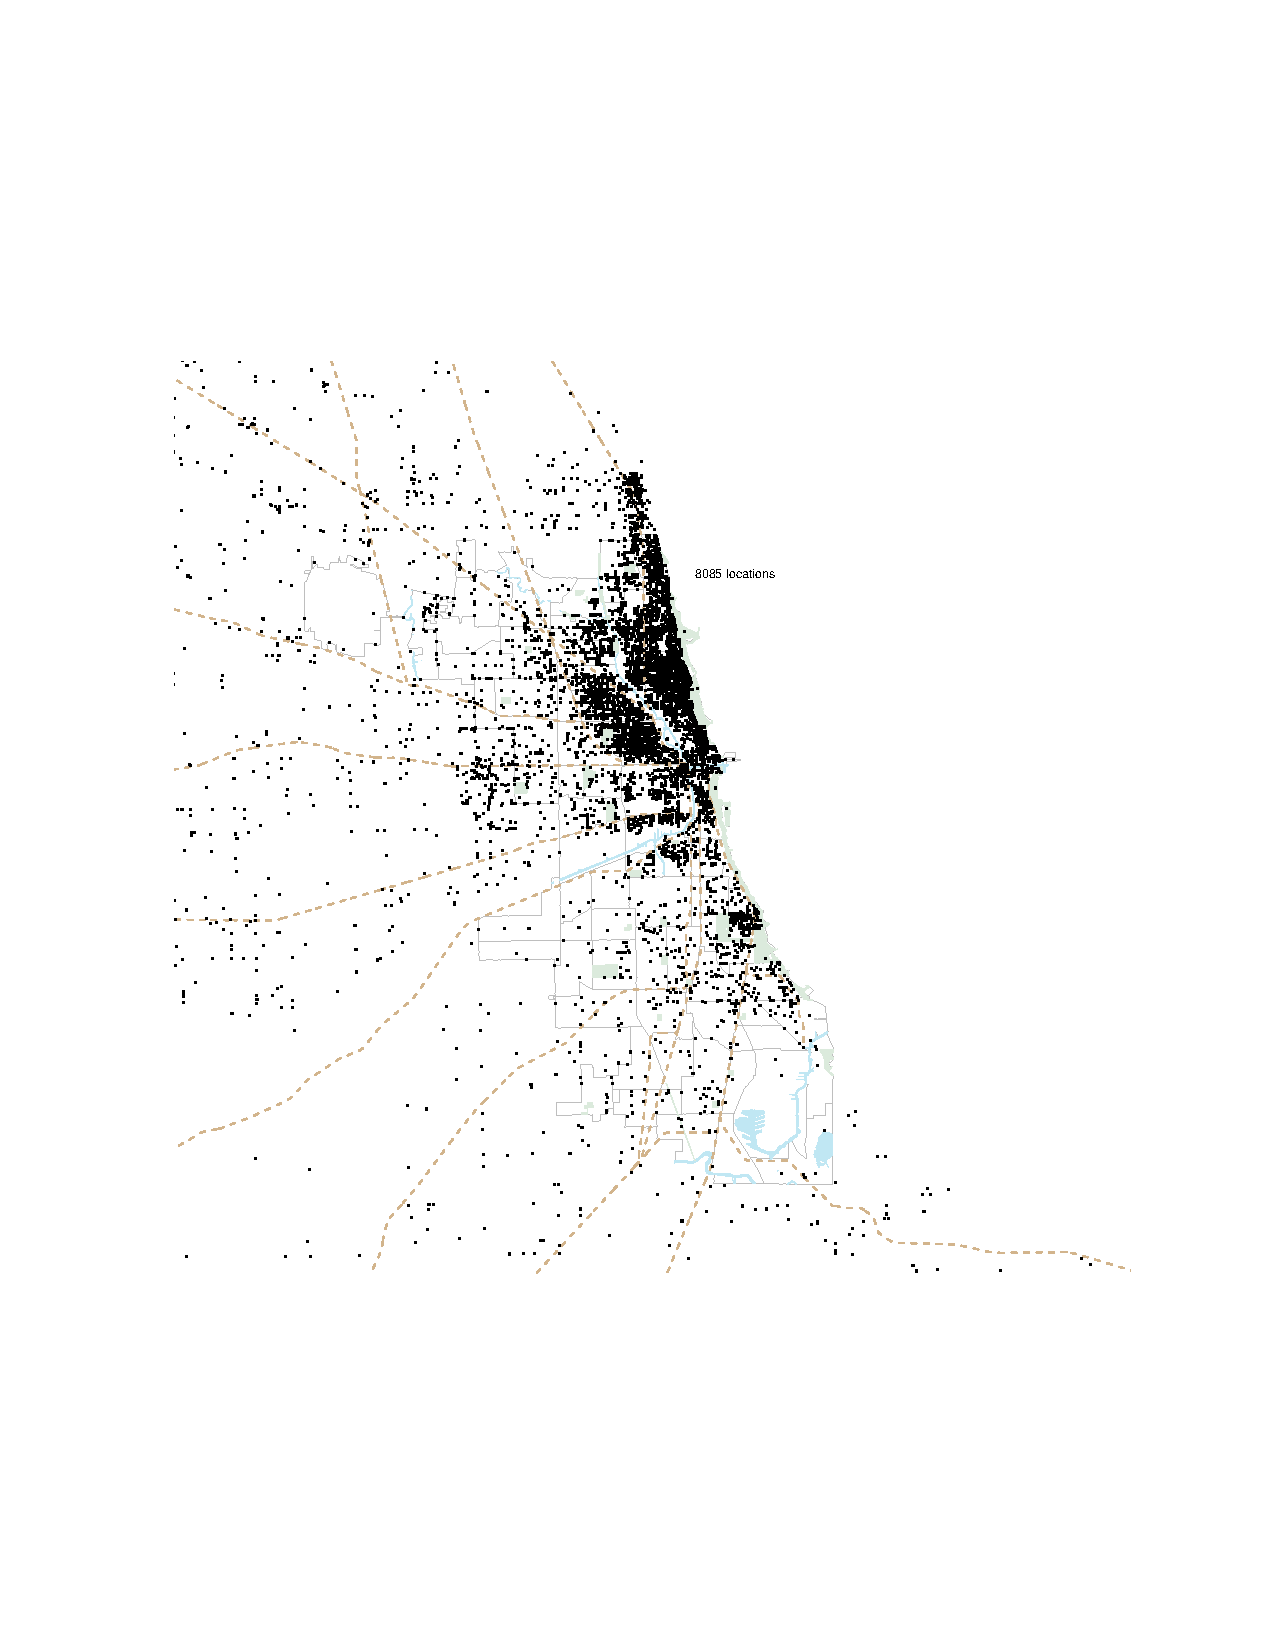
\includegraphics[width=\paperwidth]{./presentation_images/test2.pdf}
      };
    \end{tikzpicture}
  \end{frame}
}
}

I'm doing work right now to validate the Craigslist label as
reasonable proxy for the question we really want ``What is the name of
this part of Chicago.'' That question, or it's analog has been asked
on few scientifically sampled surveys, and I'm working to get that
data now.

Anyway, the point I want to make now is that it may be plausible to
use naming as a way to help define neighborhoods. But, I don't think
the standard for a good definition of a neighborhood should whether it
has a name, but whether residents can recognize the area as distinct.

\againframe<4>{valid_neighborhoods}
\begin{figure}[h!]
\centering
\includeslide[height=5cm]{valid_neighborhoods<4>}
\end{figure}

I'll leave it for another time to talk about how we can deploy these
qualities of valid neighborhood. Today, I'd like to hear your thoughts
about whether these are the kinds of things we want out for
neighborhoods or for other valid social aggregations. If we replace
some terms, do these qualities still seem reasonable?

\mode<presentation> {
  \begin{frame}<4>[label=valid_aggregations]
    Qualities of Valid Aggregations
    \begin{itemize}
    \item[]<1-> Aggregations should respect the topography of an
      underlying network
    \item[]<2-> Measures of aggregate-scale social processes should
      be relatively homogeneous within aggregations.
    \item[]<3-> Aggregations should move as a unit.
    \item[]<4-> People should recognize aggregations relevant to them.
    \item[]<5-> Aggregations should be elemental or composed of elements
    \item[]<6-> Aggregations should be permitted to not exist
    \end{itemize}
  \end{frame}
}


\againframe<6>{valid_aggregations}
\begin{figure}[h!]
\centering
\includeslide[height=5cm]{valid_aggregations<6>}
\end{figure}

\end{document}

